% Choose one to switch betweeen slides and handout
%\documentclass[]{beamer}
\documentclass[handout]{beamer}

% Video Meta Data
\title{Bitcoin, Blockchain and Cryptoassets}
\subtitle{Introduction to Cryptography: Hash Functions}
\author{Prof. Dr. Fabian Schär}
\institute{University of Basel}

% Config File
% Packages
\usepackage[utf8]{inputenc}
\usepackage{hyperref}
\usepackage{gitinfo2}
\usepackage{tikz}
\usepackage{amsmath}
\usepackage{bibentry}
\usepackage{xcolor}
\usepackage{colortbl} % Add colour to LaTeX tables
\usepackage{caption}
\usepackage[export]{adjustbox}
\usepackage{pgfplots} \pgfplotsset{compat = 1.17}

% Color Options
\definecolor{highlight}{rgb}{0.65,0.84,0.82}
\definecolor{focus}{rgb}{0.72, 0, 0}

% Beamer Template Options
\beamertemplatenavigationsymbolsempty
\setbeamertemplate{footline}[frame number]
\setbeamercolor{structure}{fg=black}
\setbeamercolor{footline}{fg=black}
\setbeamercolor{title}{fg=black}
\setbeamercolor{frametitle}{fg=black}
\setbeamercolor{item}{fg=black}
\setbeamercolor{}{fg=black}
\setbeamercolor{bibliography item}{fg=black}
\setbeamercolor*{bibliography entry title}{fg=black}
\setbeamertemplate{items}[square]
\setbeamertemplate{enumerate items}[default]
\captionsetup[figure]{labelfont={color=black},font={color=black}}
\captionsetup[table]{labelfont={color=black},font={color=black}}

\setbeamertemplate{bibliography item}{\insertbiblabel}

% Link Icon Command
\newcommand{\link}{%
    \tikz[x=1.2ex, y=1.2ex, baseline=-0.05ex]{%
        \begin{scope}[x=1ex, y=1ex]
            \clip (-0.1,-0.1)
                --++ (-0, 1.2)
                --++ (0.6, 0)
                --++ (0, -0.6)
                --++ (0.6, 0)
                --++ (0, -1);
            \path[draw,
                line width = 0.5,
                rounded corners=0.5]
                (0,0) rectangle (1,1);
        \end{scope}
        \path[draw, line width = 0.5] (0.5, 0.5)
            -- (1, 1);
        \path[draw, line width = 0.5] (0.6, 1)
            -- (1, 1) -- (1, 0.6);
        }
    }

% Read Git Data from Github Actions Workflow
% Defaults to gitinfo2 for local builds
\IfFileExists{gitInfo.txt}
	{\input{gitInfo.txt}}
	{
		\newcommand{\gitRelease}{(Local Release)}
		\newcommand{\gitSHA}{\gitHash}
		\newcommand{\gitDate}{\gitAuthorIsoDate}
	}

% Custom Titlepage
\defbeamertemplate*{title page}{customized}[1][]
{
  \vspace{-0cm}\hfill
\includegraphics[width=2.5cm]{../config/logo_cif}
  
\includegraphics[width=1.9cm]{../config/seal_wwz}
  \\ \vspace{2em}
  \usebeamerfont{title}\textbf{\inserttitle}\par
  \usebeamerfont{title}\usebeamercolor[fg]{title}\insertsubtitle\par  \vspace{1.5em}
  \small\usebeamerfont{author}\insertauthor\par
  \usebeamerfont{author}\insertinstitute\par \vspace{2em}
  \usebeamercolor[fg]{titlegraphic}\inserttitlegraphic
    \tiny \noindent \texttt{Release Ver.: \gitRelease}\\ 
    \texttt{Version Hash: \gitSHA}\\
    \texttt{Version Date: \gitDate}\\ \vspace{1em}
  \link \href{https://github.com/cifunibas/Bitcoin-Blockchain-Cryptoassets/blob/main/slides/intro.pdf}
  {Get most recent version}\\
  \link \href{https://github.com/cifunibas/Bitcoin-Blockchain-Cryptoassets/blob/main/slides/intro.pdf}
  {Watch video lecture}\\ \vspace{1em}
  License: \texttt{Creative Commons Attribution-NonCommercial-ShareAlike 4.0 International}\\\vspace{2em}
  
\includegraphics[width = 1.2cm]{../config/license}
}

% tikzlibraries
\usetikzlibrary{decorations.pathreplacing}
\usetikzlibrary{decorations.markings}
\usetikzlibrary{positioning}

%caption font
\captionsetup{font=footnotesize}


%%%%%%%%%%%%%%%%%%%%%%%%%%%%%%%%%%%%%%%%%%%%%%
%%%%%%%%%%%%%%%%%%%%%%%%%%%%%%%%%%%%%%%%%%%%%%
\begin{document}

\thispagestyle{empty}
\begin{frame}[noframenumbering]
	\titlepage
\end{frame}

%%%
\begin{frame}{What Is a Hash Function?}

Deterministic algorithm (\color{focus}function, $H()$\color{black}) that maps data of quasi-arbitrary size (\color{focus}pre-image, $m$\color{black}) to fixed-length bit string (\color{focus}hash value, $h$\color{black}).

	\begin{align}
		h = H(m)
		\label{eq:hash_function}
	\end{align}
	\vspace{1em}
	
\uncover<1->{Example of a simplified hash function:

	\begin{align}
		h = m \: \mod \: 12
		\label{eq:simple_hash_function}
	\end{align}}

This example accepts any numeric pre-image $m$ and returns a corresponding hash value $h$ $\in \{0,...,11\}$.
	
\end{frame}

%%%	

%%%
\begin{frame}{Simple Hash Functions: Checksums}

Checksums find many applications to detect human errors in data entry or faulty / incomplete data transmission.

\vspace{1em} 
\uncover<1->{IBAN Example:

		\begin{figure}[h]
  			\center
			    

\begin{tikzpicture}[scale = 0.67]

	\draw 			(0,1) node [right] {\LARGE CH 56 0483501 2345678009};
	
	\draw [focus] 	(0.2,1.6) node [left]{} -- 
					(1.35,1.6) node [midway,above] {\footnotesize \color{focus} Country Code};
					
	\draw [focus, thick] 	(1.6,0.4) node [left]{} -- 
							(2.45,0.4) node [midway,below] {\footnotesize \color{focus} \textbf{Checksum}};
							
	\draw [focus] 	(2.75,1.6) node [left]{} -- 
					(5.7,1.6) node [midway,above] {\footnotesize \color{focus} Bank Code};
					
	\draw [focus] 	(6,1.6) node [left]{} -- 
					(10.3,1.6) node [midway,above] {\footnotesize \color{focus} Account No.};
	
	\draw [focus] 	(2.75,0.4) node [left]{} -- 
					(10.3,0.4) node [midway,below] {\footnotesize \color{focus} BBAN};
					
	
\end{tikzpicture}

		\end{figure}

\footnotesize Steps:
	\begin{itemize}
		\item Take BBAN and append Country Code and 00 (empty checksum)
		\item Translate characters of country code into 9 + \texttt{<position in alphabet>}
		\item Perform mod97 operation and subtract from 98 to arrive at checksum
		\item e.g., $98 - 4835012345678009121700 \mod 97 = 56$
	\end{itemize}}
	
\end{frame}
%%%	

%%%
\begin{frame}{Further Examples and Limitations}

\textbf{Other checksum examples:}
	\begin{itemize}
		\item Credit Cards
		\item Vehicle Identification Numbers in US and Canada
		\item Radio protocols (often modulo on bytes)
		\item Communication (parity bits)
	\end{itemize}

\vspace{1em}
\uncover<1->{Purpose to \textbf{detect accidents}, not \textbf{prevent attacks}:
\begin{center}
CH\color{focus}56\color{black}04835012345678009 vs. CH\color{focus}56\color{black}048350123456\color{focus}877\color{black}09
\end{center}}


$\Rightarrow$ For security purposes, simple hashes are of limited use
	
\end{frame}
%%%	

%%%
\begin{frame}{Cryptographic Hash Functions}

Additional criteria:
	\begin{enumerate}
		\item Approximately uniform hash value distribution
		\item Quick to compute for any given pre-image
		\item Trap-door: Infeasible to generate pre-image from hash value
		\item Avalanche effect: Small change in input results in totally different output
		\item Very low collision probability: Unlikely that two pre-images generate the same hash value.
	\end{enumerate}
	\vspace{1em}

\uncover<1->{In Bitcoin context, the functions \color{focus}SHA2.256 \color{black} (in short SHA256) and \color{focus}RIPEMD160 \color{black}are used. Both satisfy the above criteria.}
	
\end{frame}
%%%	

%%%
\begin{frame}{Avalanche Effect with SHA2}

\begin{center}
$SHA256(<$\textit{pre-image}$>)$
\end{center}

This is the pre-image

$\Rightarrow$ \footnotesize 5e13fffedd642aaddea7872463fd44d8b8a336cb822ebd4c12d9e6282c88cea8 \normalsize
\vspace{1em}

\color{focus}t\color{black}his is the pre-image

$\Rightarrow$ \footnotesize \color{focus}aba56d7c281f8d\color{black}a\color{focus}cb1076baed182538d2ce21494075f7377982bf9d5d0\color{black}8\color{focus}e6ccf\color{black} \normalsize
\vspace{1em}

\begin{columns}[T]
	\begin{column}{0.35\textwidth}
		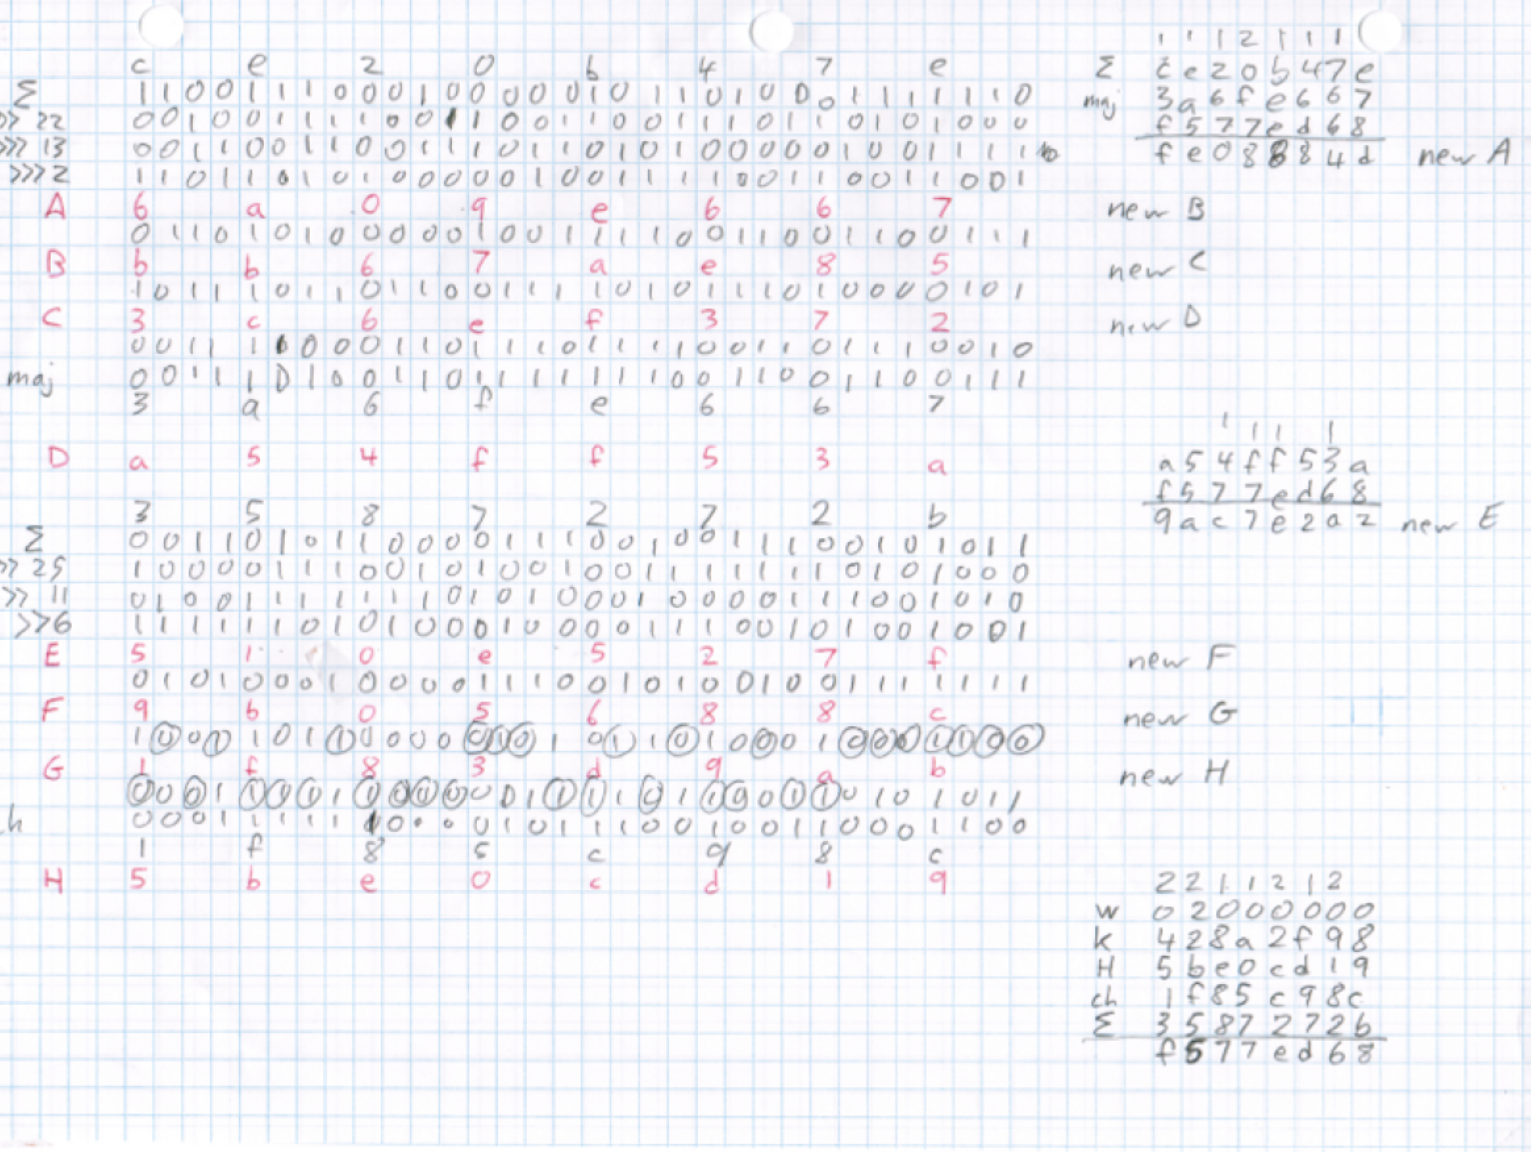
\includegraphics[width = 4 cm, frame]{../assets/images/manual_hashing_video.png}
	\end{column} %\hfill
	\begin{column}{0.65\textwidth}
		\begin{itemize}
			\item Nonlinarity due to choice, majority, mod, rotation and shifting. operations
			\item Efficient for computers vs. 0.67 hashes / day by hand.
			\item \link \href{https://www.youtube.com/watch?v=y3dqhixzGVo}{Manual calculation video}.
		\end{itemize}
	\end{column}
\end{columns}

	
\end{frame}
%%%	

%%%
\begin{frame}{Low Collision Probability}

Due to the fixed size of $h$, the corresponding hash function $H()$ can only produce a finite set of distinct hashes.
\vspace{1em}

SHA256:
	\begin{itemize}
		\item Almost all known combinations of 256 Bits, i.e.,  $2^{256}$ $h$
		\item In base 10, this is any number between 1 and 115'792'089' 237'316'195'423'570'985'008'687'907’852'837'564'279'074' 904'382'605'163'141'518'161'494'336.
	\end{itemize}
\vspace{1em}

\uncover<1->{Probability of a hexadecimal hash with certain characteristics:\\
\vspace{0.5em}
\tiny 
$P(h \leq \color{focus}0\color{black}FFFFFFFFFFFFFFFFFFFFFFFFFFFFFFFFFFFFFFFFFFFFFFFFFFFFFFFFFFFFFFF) = \dfrac{1}{16}$\\
\vspace{1em}
$P(h \leq \color{focus}00\color{black}FFFFFFFFFFFFFFFFFFFFFFFFFFFFFFFFFFFFFFFFFFFFFFFFFFFFFFFFFFFFFF) = \left( \dfrac{1}{16} \right)^{2} $

\normalsize}

	
\end{frame}
%%%	

%%%
\begin{frame}{Example in Bitcoin Context}

How much time would it take to find a pre-image that generates a specific hash using the cryptographic hash functions applied in Bitcoin with a trial and error approach?

\vspace{1em}

\uncover<1->{\textbf{Assumptions:}
		\begin{itemize}
			\item Computer runs 24/7
			\item Hashrate of 60b/second
		\end{itemize}

\vspace{1em}}
	
\uncover<2->{\textbf{Outcome:\\
 \color{focus}1\% \color{black}} chance to find a specific hash \textbf{within $7 \cdot 10^{27}$ years}.}

	
\end{frame}
%%%	


\begin{frame}%[allowframebreaks]
\frametitle{References and Recommended Reading}

		\begin{columns}[T]
			\begin{column}{0.1\textwidth}
					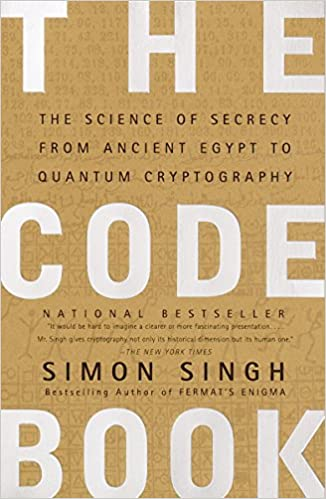
\includegraphics[width = 1.65cm, frame]{../assets/images/singh_cover}
			\end{column} %\hfill
			\begin{column}{0.8\textwidth}
				\textbf{The Code Book} \\ 
				Simon Singh \\
				\texttt{ISBN: 978-0385495325}
			\end{column}
		\end{columns}
	%
	\vspace{1.5em}
	%
	\uncover<1->{
		\begin{columns}[T]
			\begin{column}{0.1\textwidth}
					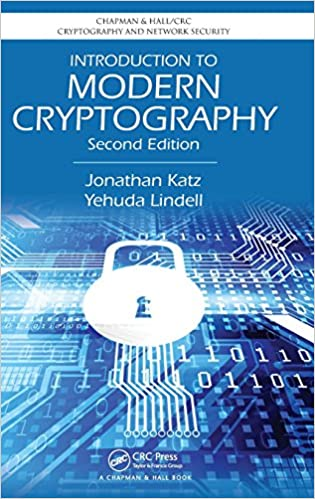
\includegraphics[width = 1.65cm, frame]{../assets/images/katz_lindell_cover}
			\end{column} %\hfill
			\begin{column}{0.8\textwidth}
				\textbf{Introduction to Modern Cryptography} \\ 
				Jonathan Katz and Yehuda Lindell \\
				\texttt{ISBN: 978-1466570269}
			\end{column}
		\end{columns}
	}
	%
	\vspace{1.5em}
	%
	\uncover<2->{
		\begin{columns}[T]
			\begin{column}{0.1\textwidth}
					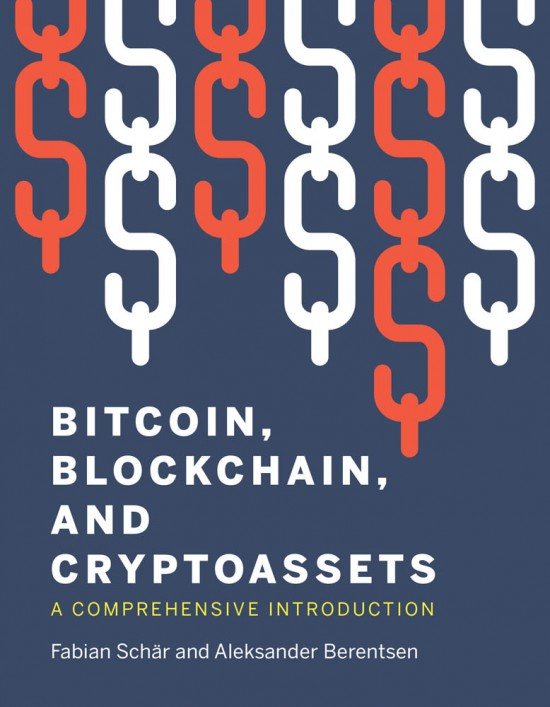
\includegraphics[width = 1.65cm, frame]{../assets/images/schaer_berentsen_cover}
			\end{column} %\hfill
			\begin{column}{0.8\textwidth}
				\textbf{Bitcoin, Blockchain and Cryptoassets} \\ 
				Fabian Schär and Aleksander Berentsen \\
				\texttt{ISBN: 978-0262539166}
			\end{column}
		\end{columns}
	}

\end{frame}


\end{document}
